\documentclass{article}
\usepackage[utf8]{inputenc}
\usepackage[margin=1in,left=1.5in,includefoot]{geometry}
\usepackage{booktabs}
\usepackage{graphicx}
\usepackage{hyperref}
\usepackage{wrapfig}
\usepackage{float}
\usepackage{amsmath}
\usepackage{amssymb}
\usepackage[galician]{babel}
\usepackage[most]{tcolorbox}
\usepackage{listings}
\usepackage{lmodern}
\usepackage{xcolor}
\usepackage{caption}
\usepackage{pgfornament}

\newtcolorbox{clibox}{
  colback=gray!10,    % light gray background
  colframe=gray!50,   % gray border
  boxrule=0.5pt,      % border thickness
  arc=2pt,            % rounded corners
  left=6pt,
  right=6pt,
  top=6pt,
  bottom=6pt,
  fontupper=\ttfamily % monospaced font
}


% Header & Footer Stuff

\usepackage{fancyhdr}
\pagestyle{fancy}
\lhead{\emph{Visión por Computador Aplicada}}
\rhead{614G030332425}
% \fancyfoot{}
% \lfoot{Pablo Chantada Saborido \& José Romero Conde}
% \fancyfoot[R]{}

% The Main Document
\begin{document}
	\begin{center}
		\LARGE\bfseries PRÁCTICA II\\
		\small Pablo Chantada Saborido \& José Romero Conde
	\end{center}
	
	\begin{center}
		\pgfornament[width=0.8\linewidth,color=black]{88}
	\end{center}
	
\vspace*{300pt}
	
\begin{figure}[H]
	\centering
	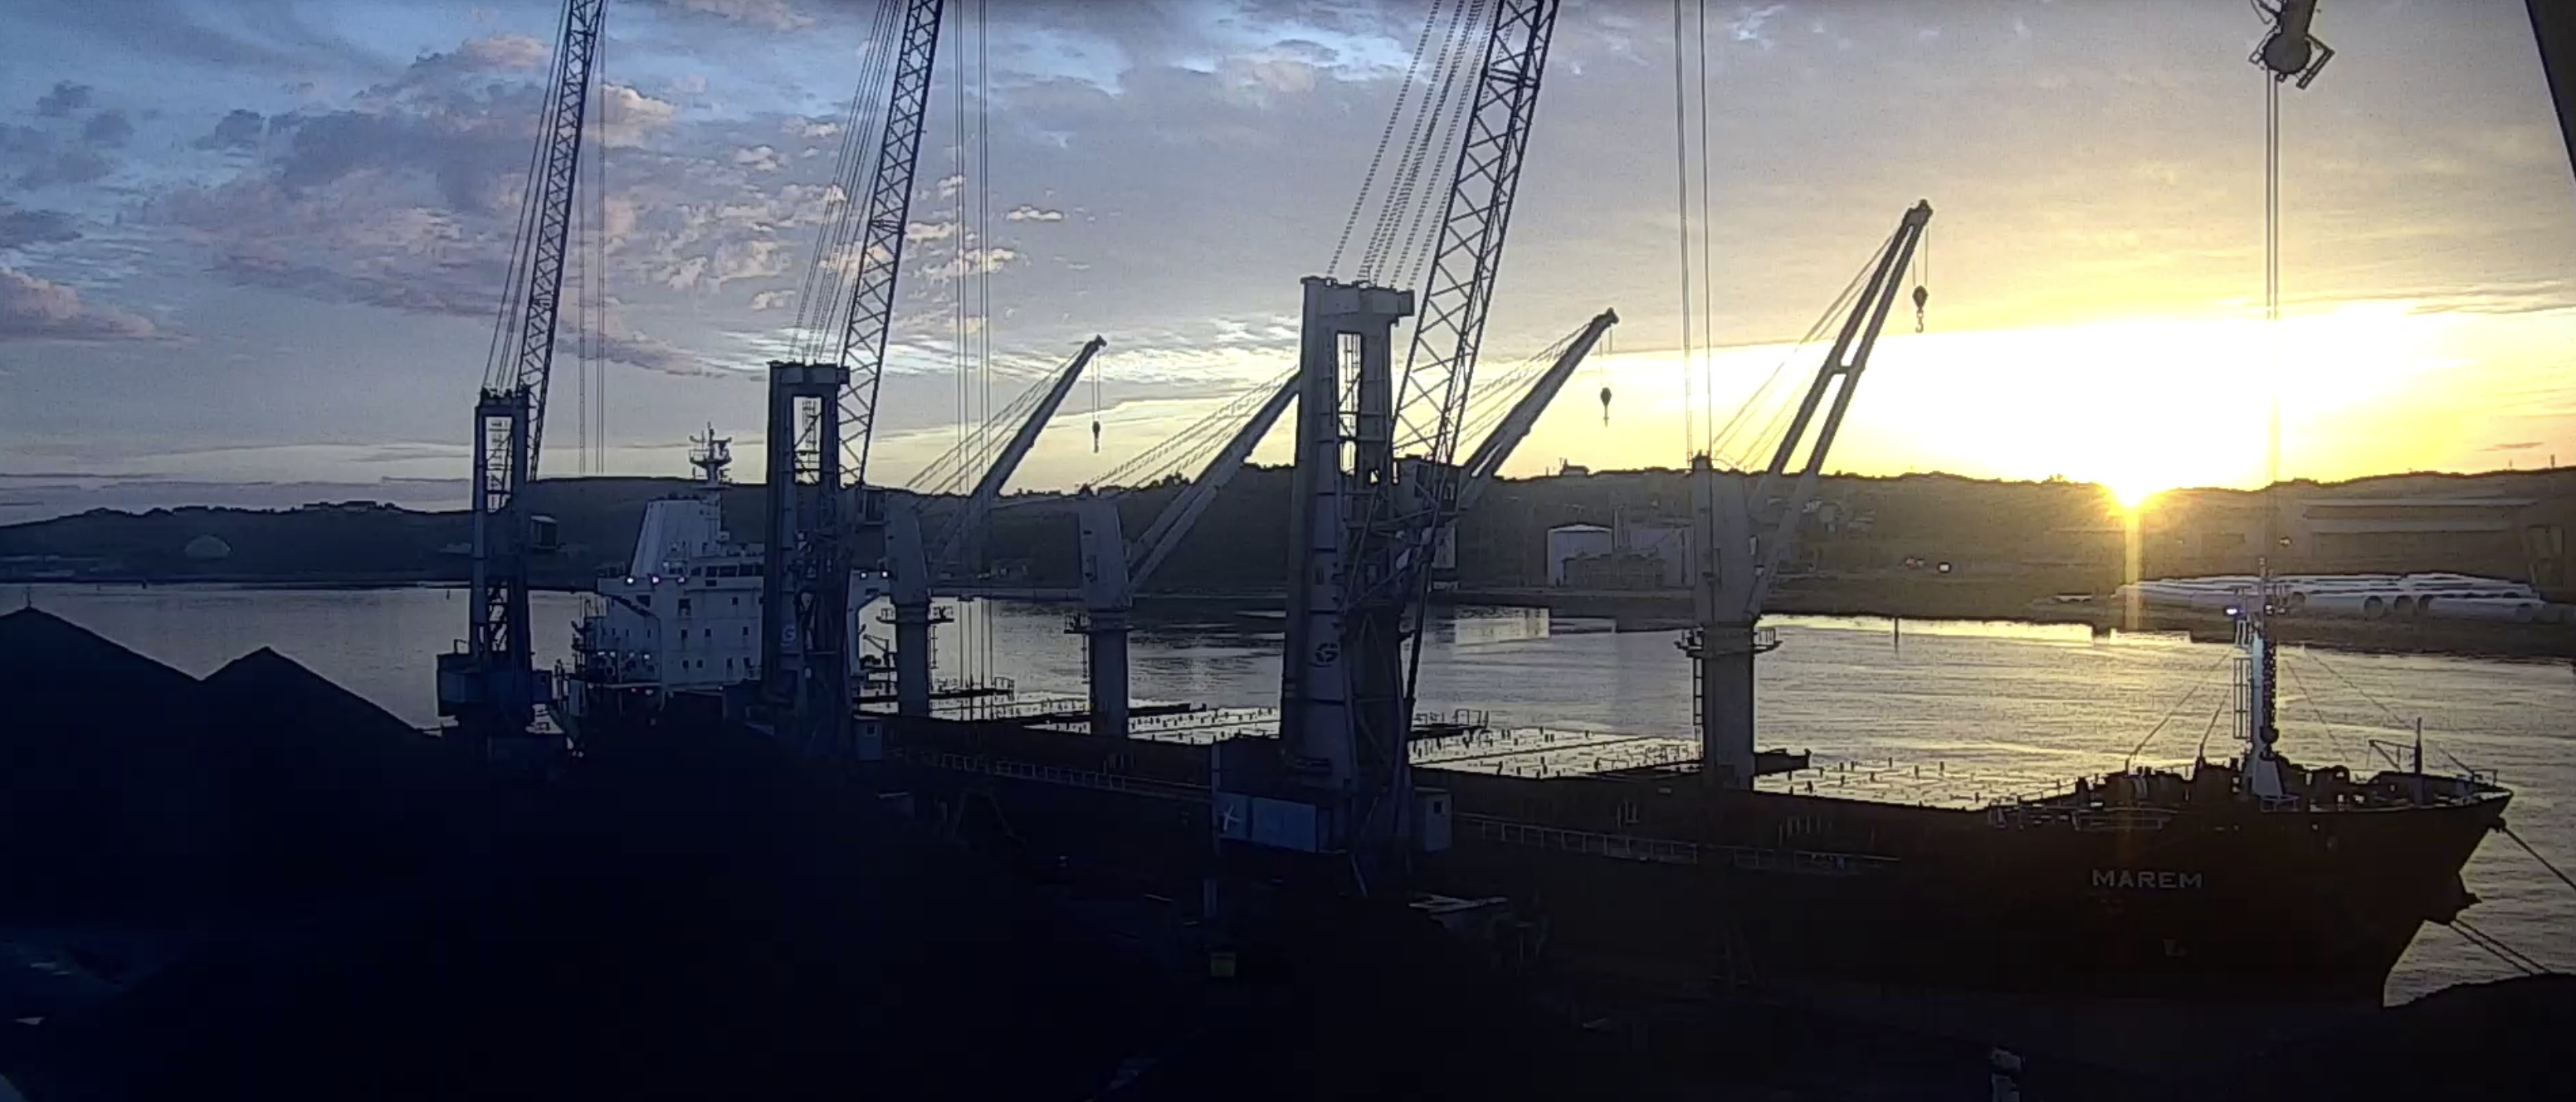
\includegraphics[width=0.7\linewidth]{figuras/portada.jpg}
	\label{fig:portada}
\end{figure}
	
\thispagestyle{empty}
	
\newpage

\tableofcontents

\newpage
	
	
\section{Introdución}

Esta práctica supuxo todo un reto para nós. O conxunto de datos foi especialmente difícil polos seguintes motivos:
\begin{itemize}
	\item \textbf{Escaseza de datos.} Acostumados a miles (MNIST) ou centos (SmartPorts) de imaxes, contar con só decenas delas supuxo unha dificultade no problema a resolver. Isto débese a que a nosa rede ten que aprender moito de cada imaxe, e saber extrapolar o aprendido a imaxes que nunca viu. Nada sinxelo.
	\item \textbf{Alta variabilidade.} Se foran poucos datos pero a realidade fose sempre moi parecida, non habería tanto problema, a cuestión é que dunha imaxe a outra pode haber pouco que teñan en común. As hai que a parede ocular é fina e ten unha fendedura, as hai sen fendedura mais cun gran vaso, as hai sen fendedura e con múltiples vasos... isto é para nós un problema porque o fluxo óptico \emph{existe} dun xeito distinto en cada imaxe de OCT. Polo tanto, a nosa rede debe aprender todas esas variacións con poucos exemplos.
	\item \textbf{Imperfección da supervisión.} Aínda que poderíamos ter feito un AutoEncoder para cerciorarnos dunha boa representación \emph{latente}, limitámonos ao uso das máscaras para propagar o sinal de erro. Ao non seren perfectas e consistentes as etiquetas (zonas dun certo nivel de gris rodeadas dun capilar, en unhas máscaras representábase o capilar e noutras non), non podemos esperar que o noso algoritmo o sexa. Ademais, está baseándose exclusivamente en exemplos mentres que un médico razoa e delibera en base aos seus coñecementos teóricos e de dominio. A nosa rede non pode facer tal cousa.


\begin{figure}[H]
	\centering
	\includegraphics[width=\linewidth]{figuras/defecto_medico.png}
	\label{fig:defecto_medico}
\end{figure}

Arriba pode verse un exemplo que nos chamou a atención. Na área rodeada cun círculo violeta, na imaxe orixinal pódense ver tres \emph{paredes}, en cambio o GT só respectou a da dereita de todo e a do medio suxeriuna pero non a rematou, e a da esquerda, o GT nin a asomou. En cambio, a nosa rede si tivo en conta a primeira parede. Este exemplo mostra que o GT non é perfecto e que perseguilo pode ofrecer bos resultados pero só ata un punto. Por outro lado, no hospital cando for a usarse a rede, igual non importa se segmenta ben esa parede, nós non podemos sabelo pero unha revisión dun blog médico \cite{paxinaOCT} suxire que probablemente ese nivel de detalle non sexa importante.

\end{itemize}

Para afrontar o problema, por tanto, armámonos cunha serie de técnicas e trucos aprendidos nesta asignatura, en Aprendizaxe Profundo e mais en Principios de Visión por Computador. Son os seguintes:
\begin{itemize}
	\item \textbf{Canles adicionais de entrada.} A rede ten que aprender que é o fluxo óptico desde cero, sen saber que é un bordo ou un círculo. Non lle pasa o mesmo aos médicos, que cando empezan na oftalmoloxía xa teñen un adestrado sistema de percepción visual. Polo tanto, para axilizar este proceso, ademais da imaxe en branco e negro $\mathcal{I}$ (unha canle) decidimos acompañala dos $\phi_i(\mathcal{I})$ onde os $\phi_i$ son algoritmos de procesado de imaxe. Inicialmente escollemos Canny \cite{canny1986computational}, Sobel, Laplaciano e Frangi \cite{frangi1998multiscale}. Do último tiñamos altas esperanzas por estar tamén orientado ao ámbito médico mais aínda despois dunha considerable procura de hiperparámetros decidimos descartalo para, finalmente, só quedarnos con Canny. Unha xustificación desta decisión é a imaxe de abaixo. 

\begin{figure}[H]
	\centering
	\includegraphics[width=\linewidth]{figuras/canles.png}
	\label{fig:canles}
\end{figure}


\item \textbf{Aumento de datos.} Fundamentalmente baseámonos nas suxestións do propio artigo da UNet \cite{ronneberger2015u}, é dicir: transformacións afíns e elásticas. Coas primeiras foi relativamente doado atopar hiperparámetros apropiados pero as segundas foi máis difícil, en cambio (ao estaren deseñadas para un contexto de segmentación médica) ofreceron moi bos resultados. Finalmente atopamos $\alpha = 500$ e $\sigma = 20$ axeitados. Ademais, para estas dúas transformacións, ao seren relativamente \emph{agresivas}, atopamos que é mellor non transformar sempre (para darlle á rede uns poucos exemplos inalterados e aprenda deles). En concreto aplicamos cada unha delas cunha probabilidade de 0.7, polo tanto, para unha imaxe, a probabilidade de ser alterada por ambas transformacións é de $\approx 0.5$. Ademais destas dúas, aplicamos (malia observar pouca diferenza) volteos horizontais, deformacións na cor (\emph{color jitter}), variacións no enfoque e ruído gaussiano aditivo. O efecto da totalidade das transformacións sobre un subconxunto das imaxes do conxunto de datos vese abaixo.

\begin{figure}[H]
	\centering
	\includegraphics[width=\linewidth]{figuras/aumento_datos.png}
	\label{fig:AD}
\end{figure}


Se ben pode parecer \emph{leve}, aumentos de datos máis agresivos non vían a luz da converxencia. Podemos dicir que a configuración de hiperparámetros do aumento de datos está fortemente baseada na experimentación. Comentar que tamén probamos a recortar as imaxes centrando a máscara como forma de aumento de datos pero encontramos que empeoraba o rendemento; ese tipo de cousas poden ser útiles para tarefas de clasificación pero como a segmentación depende da escala en concreto e no conxunto de datos sempre era relativamente a mesma escala, facer grandes variacións nese sentido pode (como temos visto) empeorar o rendemento da rede.

\item \textbf{Posprocesado das máscaras.} Aínda que non diferenciables, e por tanto non contribuían ao sinal de erro do adestramento do algoritmo, decidimos aplicar unha serie de transformacións sobre as máscaras para achegarse máis ás reais. Pulindo detalles de xeito que, se un oftalmólogo tivera que usar o noso sistema, certas impurezas corrixibles non o molestarían. En concreto, axudámonos do operador morfolóxico de peche.

\begin{figure}[H]
	\centering
	\includegraphics[width=\linewidth]{figuras/peche.png}
	\label{fig:peche}
\end{figure}

Comentar, non obstante, que por non ser o obxectivo da práctica o resultado final senón o adestramento da rede en si mesma, limitámonos a unha primeira idea de só aplicar peche, mais de seguro poderían implementarse máis e mellores alternativas.

\item \textbf{\emph{Trucos} no adestramento da rede.} Para asegurar converxencia e acelerar o adestramento usamos Dropout \cite{srivastava2014dropout} como regularización e AdamW \cite{loshchilov2019decoupled} como optimizador que tamén implementa regularización a través dos pesos. Estes dous elementos permitiron que se propagase axeitadamente o sinal de erro na rede, que nalgúns experimentos fixemos moi grande. Adicionalmente, adicando un subconxunto dos datos a \emph{validación}, implementamos \emph{EarlyStopping} con paciencia na perda en validación e máis un xestor do paso de aprendizaxe que, tamén, tiña paciencia coa perda en validación. Estes dous compoñentes fixeron dinámicos parámetros que, de seren estáticos e sempre iguais, non permitirían aprender con éxito ás redes porque as redes máis grandes precisan (en xeral) máis épocas, e un único paso de aprendizaxe pode estar ben pero non adoita explotar todo o potencial dunha rede dada. Como última consideración, implementamos unha función de perda combinada, do seguinte xeito: \[\mathcal{L} = \alpha_{BCE} \times \mathcal{L}_{BCE} + \alpha_{FOCAL} \times \mathcal{L}_{FOCAL} + \alpha_{DICE} \times \mathcal{L}_{DICE} + \alpha_{IOU} \times \mathcal{L}_{IOU}\] onde nós fixamos $\alpha_{BCE} = 0.7$, $\alpha_{FOCAL} = 0.2$, $\alpha_{DICE} = 0.4$, $\alpha_{IOU} = 0.7$. Eses coeficientes fixáronse a partir de observar as primeiras gráficas de adestramento. Abaixo pódese ver unha gráfica coa función de perda aquí descrita. 

\begin{figure}[H]
	\centering
	\includegraphics[width=\linewidth]{figuras/CU_adTrue_batch10_proc7_canles32_prof4_lr0.001_factocurva_perdida.jpg}
	\label{fig:perdida_funcion}
\end{figure}

\end{itemize}

\section{O noso formulamento}

Despois de ter feito a práctica anterior, recoñecemos as vantaxes dun bo formulamento inicial, tanto no nivel conceptual e máis de \emph{visión} como no nivel técnico e máis de \emph{programación}. É por isto que desde un primeiro momento formulamos a práctica como un todo, por tanto, non fixemos primeiro un \emph{Baseline} e logo experimentos e melloras sobre iso; en vez diso, desde un primeiro momento formulamos na parte de programación a interface necesaria para, logo, facer experimentos e atopar que combinación ofrecen bos resultados. Comentamos agora, aspectos nos que fixemos probas e as nosas conclusións:

\begin{itemize}
	\item \textbf{Tamaño das imaxes.} As primeiras redes que adestramos (poderíamos consideralas en parte, \emph{baselines}) empregaban imaxes relativamente pequenas (por custo computacional) e moi rectangulares (200 píxeles por 500), porque observando as imaxes vimos que tiñan un ratio moi pronunciado. Isto pódese comprobar cos seguintes comandos de UNIX (no directorio das imaxes):


\begin{tcolorbox}[colback=gray!10!white, colframe=gray!50!black, 
  boxrule=0.5pt, arc=2pt, left=4pt, right=4pt, top=2pt, bottom=2pt,
  fontupper=\ttfamily\small]
\$ identify * | awk '\{print \$3\}' | awk -F'x' '\{suma += \$1/\$2; n++\} END \{print ``Razón ancho-alto media:'', suma/n\}' \\
\string>>\ Razón ancho-alto media: 2.6163
\end{tcolorbox}

Posteriormente decatámonos de que para que a rede percibira propiamente as paredes do Fluxo Óptico, estas non podían ter de ancho 2 ou 3 píxeles, entón, malia seren máis computacionalmente custosos, os modelos adestrados con imaxes máis grandes ofreceron mellores resultados. Tamén decatámonos de que malia seren as imaxes moi rectangulares, a máscara sempre estaba no centro e non pagaba a pena o bordo, entón, malia saber que as imaxes eran moi rectangulares, a nosa decisión final foi de 400 por 500. 

\item \textbf{Profundidade e canles base da UNet.} Despois da lectura do artigo \cite{ronneberger2015u}, decatámonos de que a UNet, máis que un modelo en concreto, é unha concepción que pode instanciarse no xeito que o fixeron os autores, é dicir, 3 niveis de profundidade 64 canles de saída na primeira convolución, pero que facilmente pode mutar a outras configuracións. Abaixo probamos a adestrar a rede coa mesma configuración variando só as canles de entrada (4 primeiras imaxes) e vemos que, (como se suxeriu xa no 2012 \cite{imagenet}) canto máis grande é a rede mellores resultados. Tamén aproveitamos para mostrar o efecto do Dropout \cite{srivastava2014dropout} (recomendado no artigo orixinal \cite{ronneberger2015u}), que é o único que varía nas dúas imaxes de abaixo. 

\begin{figure}[htbp]
    \centering
    \begin{minipage}{0.32\textwidth}
    \centering
        \includegraphics[width=\linewidth]{figuras/8.jpg}
        \caption*{8 canles base}
    \end{minipage}
    \hfill
    \begin{minipage}{0.32\textwidth}
    \centering
        \includegraphics[width=\linewidth]{figuras/16.jpg}
        \caption*{16 canles base}
    \end{minipage}
    \hfill
    \begin{minipage}{0.32\textwidth}
    \centering
        \includegraphics[width=\linewidth]{figuras/32.jpg}
        \caption*{32 canles base}
    \end{minipage}
    \hfill
    \begin{minipage}{0.48\textwidth}
    \centering
        \includegraphics[width=\linewidth]{figuras/64.jpg}
	\caption*{64 canles base, DP = 0}
    \end{minipage}
    \hfill
    \begin{minipage}{0.48\textwidth}
    \centering
        \includegraphics[width=\linewidth]{figuras/64D.jpg}
	\caption*{64 canles base, DP = 0.1}
    \end{minipage}
\end{figure}

Os mesmos resultados poden dicirse da profundidade, ademais, a profundidade ten que ver co tamaño do campo receptivo, o cal tamén encontramos beneficioso.

\item \textbf{Aumento de datos.} Definir o aumento de datos como o temos feito tamén pode considerarse unha extensión sobre o \emph{baseline}. Abaixo móstranse dous adestramentos da mesma rede (64 canles base, 3 niveis de profundidade na UNet e Dropout de 0.05) e pódese ver que o aumento de datos esencialmente permite adestramentos máis longos, nos que a aprendizaxe ata converxencia sexa maior.


\begin{figure}[htbp]
    \centering
    \begin{minipage}{0.45\textwidth}
    \centering
        \includegraphics[width=\linewidth]{figuras/ADT.jpg}
        \caption*{Con aumento de datos}
    \end{minipage}
    \hfill
    \begin{minipage}{0.45\textwidth}
    \centering
        \includegraphics[width=\linewidth]{figuras/ADF.jpg}
        \caption*{Sen aumento de datos}
    \end{minipage}
\end{figure}

\end{itemize}

\begin{figure}[H]
	\centering
	\includegraphics[width=\linewidth]{figuras/conclusion.jpg}
	\caption{Resultados dunha execución con aumento de datos, 32 canles iniciais, 4 niveis de profundidade, ningún Dropout e un DICE en proba de 0.9 (Para proba usáronse 5 imaxes, tendo destinadas outras 5 a validación e 40 ao adestramento). }
\end{figure}

\section{Conclusións}


En primeiro lugar, o problema da segmentación en imaxes médicas presenta desafíos específicos que requiren dunha aproximación diferente dos casos aos que estamos acostumados. A escaseza de datos, a alta variabilidade entre imaxes e a imperfección das etiquetas foron os principais obstáculos que tivemos que afrontar.

A arquitectura UNet demostrou ser moi eficaz para esta tarefa, especialmente cando se configura adecuadamente en termos de profundidade e número de canles. Nos nosos experimentos, puidemos comprobar que (por desfortuna para a nosa limitada capacidade de cómputo) as redes máis grandes obteñen mellores resultados, o cal está en liña co observado noutros traballos  do campo.

O aumento de datos foi unha técnica fundamental para mellorar o rendemento do modelo, especialmente as transformacións elásticas, que xustamente foron propostas para segmentación de imaxes médicas ca UNet. Esta técnica permitiunos estender o conxunto de adestramento e mellorar a capacidade de xeneralización da rede ante variacións que sabemos que son comúns en texidos biolóxicos.

A combinación de diferentes funcións de perda proporcionou unha supervisión máis certera e permitiu obter mellores resultados que utilizando unha única métrica. Unha investigación máis exhaustiva podería usar xestores dos hiperparámetros $\alpha_i$ co tempo, pero os nosos resultados, para o tempo e alcance da práctica, resultaron ser suficientes.

A incorporación de canles adicionais de entrada, como o filtro Canny, permitiu á rede aprender características relevantes do fluxo óptico sen necesidade de partir desde cero, o que acelerou o proceso de aprendizaxe e mellorou os resultados finais. En outras palabras, permituinos non ter que empezar de cero.

En definitiva, este traballo demostra que as redes neuronais profundas, especificamente a arquitectura UNet con modificacións apropiadas, poden acadar resultados moi satisfactorios na segmentación do fluxo óptico en imaxes OCT, mesmo en escenarios con datos limitados e alta variabilidade. Os nosos mellores modelos acadaron un coeficiente DICE de 0.9 no conxunto de proba, o que suxire un alto grao de concordancia coas anotacións médicas, sobretodo considerando que seguramente un médico non consiga un 1 (e posiblemente un oftalmólogo de prácticas consiga menos ca nos) e mostra o potencial desta aproximación para aplicacións clínicas reais.



\newpage

\bibliographystyle{plain}  % or alpha, ieee, etc.
\bibliography{referencias} % No .bib extension




\end{document}
